% Setting up the LaTeX document with necessary packages
\documentclass{article}
\usepackage[margin=1in]{geometry}
\usepackage{amsmath,amsfonts}
\usepackage{parskip}
\usepackage{graphicx}
\usepackage{hyperref}
\usepackage{pdflscape} % Added for landscape orientation
\usepackage{tikz}
\usetikzlibrary{shapes.geometric, arrows.meta, positioning}
\setlength{\parindent}{0pt}

% Beginning the document
\begin{document}

% Defining the title, author, and date
\title{K-Square Programme Onboarding Agent: Enhancing Execution Team Integration}
\author{Alberto Espinosa \\ KSquare Group}
\date{1 August 2025}
\maketitle

% Providing an abstract for the document
\begin{abstract}
The K-Square Programme Onboarding Agent is an artificial intelligence system designed to streamline the onboarding process for programme execution teams following project acquisition. By combining a conversational AI interface with a visual knowledge base, the system aggregates internal and external data to deliver domain-specific insights, client profiles, and actionable recommendations. This paper presents the system’s architecture, core principles, implications, and proposed technologies, such as LangGraph and Ollama, for implementation, ensuring efficient integration within a 2–3 day timeframe.
\end{abstract}

% Introducing the system and its purpose
\section{Introduction}
The onboarding of programme execution teams post-project acquisition is a pivotal phase in project management. Traditional manual processes, reliant on knowledge transfer from sales and pre-sales teams, are often inefficient and time-consuming. The K-Square Programme Onboarding Agent addresses this challenge by automating data aggregation and insight generation, enabling rapid and effective team integration. This internal tool focuses on pre-onboarding, preparing teams before project execution begins, using a conversational interface and structured visual outputs. This paper outlines the system’s design, principles, and potential impact on enterprise workflows.

% Describing the system’s architecture and workflow
\section{System Overview}
The K-Square Programme Onboarding Agent is a closed-loop ecosystem that integrates internal data (e.g., SharePoint documents, meeting recordings) and external data (e.g., public web sources) to facilitate pre-onboarding. It combines a conversational AI for data input with a visual dashboard for team access, comprising six core components:

% Listing the system components
\begin{itemize}
    \item \textbf{Programme Setup Agent}: Guides users through a conversational interface to input project and client details, such as client name, industry, problem statement, and SharePoint links.
    \item \textbf{Domain Knowledge Agent}: Aggregates internal and external data to provide domain-specific insights, best practices, and reusable templates.
    \item \textbf{Client Profile Agent}: Builds detailed client profiles using internal documents and public data, validated by users for relevance.
    \item \textbf{Actionable Insights Agent}: Generates recommendations, summaries, and tasks to guide team preparation.
    \item \textbf{Meetings Agent}: Analyses Microsoft Teams recordings to extract action items, scope insights, and engagement metrics.
    \item \textbf{Knowledge Base}: Centralises tagged data in a visual format for team access and reference.
\end{itemize}

The system leverages structured internal repositories and a tagging system to organise outputs, ensuring scalability and accessibility for teams within a 2–3 day onboarding period.

% Illustrating the system workflow with a diagram
\subsection{System Workflow}
The system’s workflow, depicted in Figure \ref{fig:workflow}, illustrates data flow from user inputs through a conversational AI to onboarding outputs presented in a visual dashboard. Users interact with the Programme Setup Agent to provide project details, which are processed by other agents, validated, and stored in the Knowledge Base for team access.

% Placing the figure on a single landscape page
\begin{landscape}
\begin{figure}[p]
    \centering
    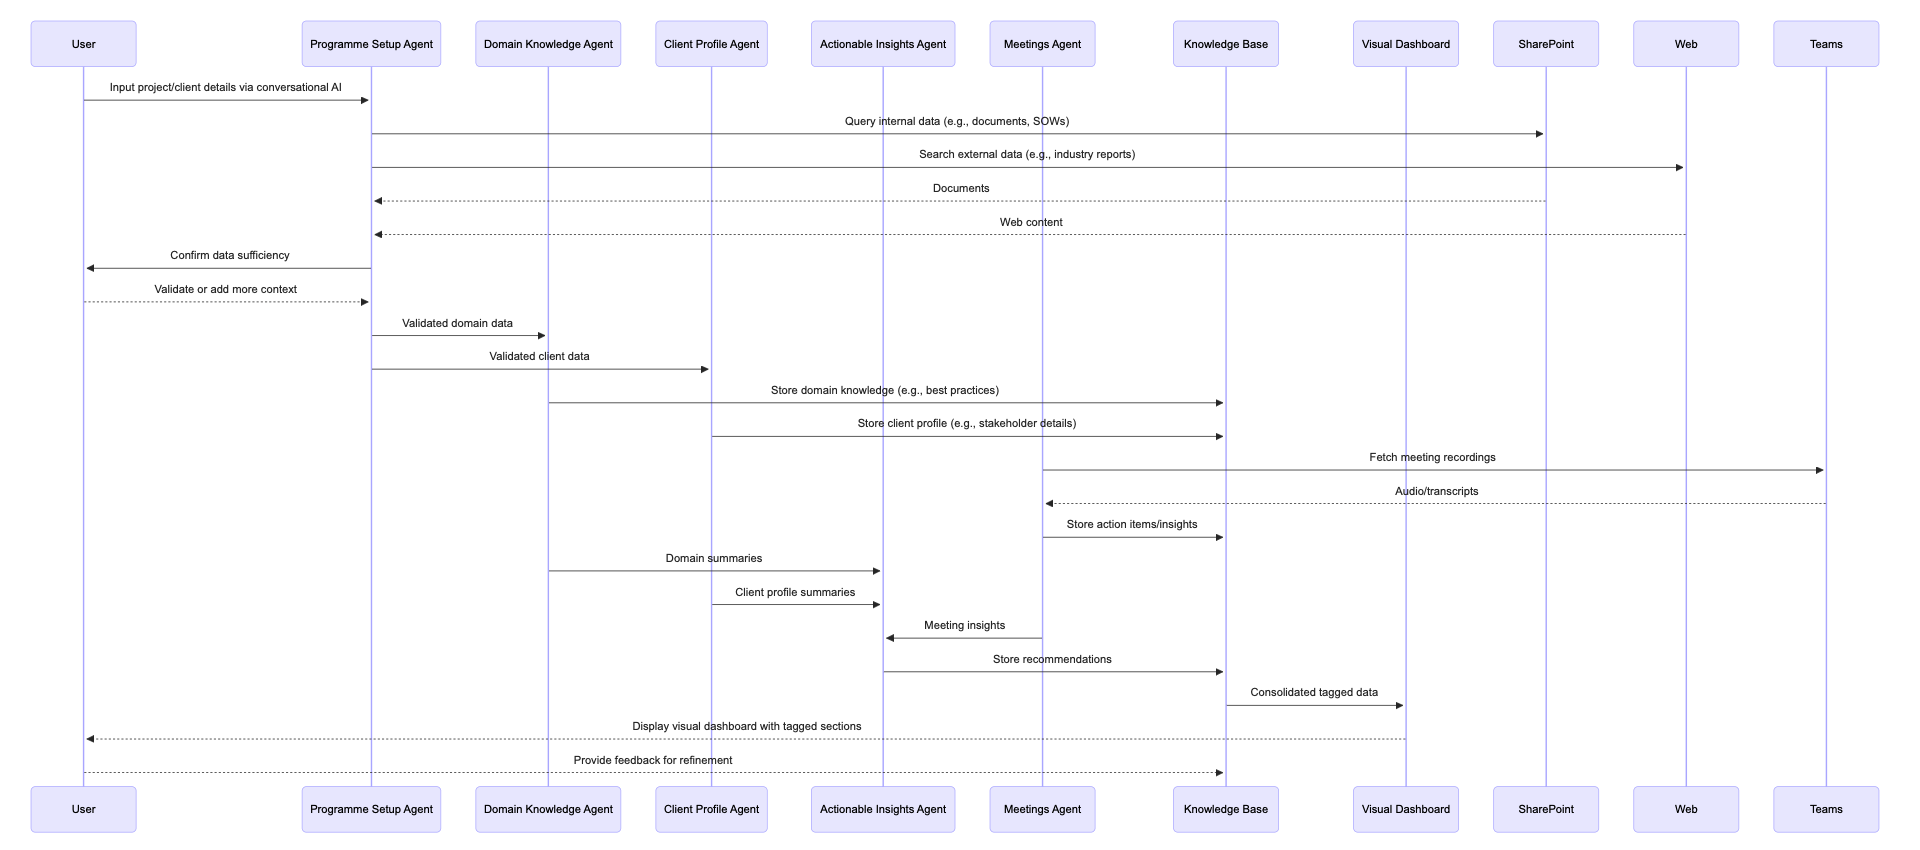
\includegraphics[width=\textwidth]{/Users/albertohernandez/Documents/projects/KS-onboarding/doc/images/workflow.png}
    \caption{Workflow of the K-Square Programme Onboarding Agent, showing conversational input and visual output.}
    \label{fig:workflow}
\end{figure}
\end{landscape}

% Outlining the core principles of the system
\section{Core Principles}
The system is guided by the following principles:
\begin{itemize}
    \item \textbf{Automation}: Automates data aggregation and insight generation to minimise manual knowledge transfer.
    \item \textbf{Conversational Interaction}: Employs a chat-based interface to simplify data input and guide users step-by-step.
    \item \textbf{Visual Organisation}: Presents information in a structured, visual format (e.g., a dashboard or board) for team accessibility.
    \item \textbf{Human Validation}: Incorporates user feedback to refine AI outputs, ensuring accuracy and relevance.
    \item \textbf{Structured Data}: Relies on organised internal repositories (e.g., SharePoint) for efficient data retrieval.
    \item \textbf{Actionable Outputs}: Delivers summaries, checklists, and recommendations to enable rapid project initiation.
\end{itemize}

% Discussing the implications of the system
\section{Implications}
The K-Square Programme Onboarding Agent offers significant benefits for programme management:
\begin{itemize}
    \item \textbf{Efficiency}: Reduces onboarding time to 2–3 days, accelerating project execution.
    \item \textbf{Scalability}: Supports multiple clients and industries through a modular, tagged data structure.
    \item \textbf{Enterprise Integration}: Aligns with tools like Microsoft Teams and SharePoint, facilitating adoption.
    \item \textbf{Team Preparedness}: Equips teams with comprehensive client and domain knowledge, enhancing client interactions.
\end{itemize}

% Highlighting the relevance of the system
\section{Relevance}
The system addresses a critical need in programme management: rapid and effective team onboarding. By automating pre-onboarding tasks and delivering structured insights, it reduces reliance on stakeholder availability and ensures consistent knowledge delivery. Its focus on internal use and pre-execution preparation aligns with enterprise priorities, optimising project initiation processes.

% Exploring architectural possibilities for implementation
\section{Architectural Possibilities}
The system’s architecture leverages agentic technologies, with LangGraph and Ollama as primary candidates, complemented by alternatives for specific tasks.

% Describing LangGraph as a framework
\subsection{LangGraph}
LangGraph, a graph-based framework for multi-agent workflows, orchestrates the system’s agents by enabling dynamic task routing. Outputs from the Domain Knowledge and Client Profile Agents feed into the Actionable Insights Agent, ensuring efficient data flow. Its flexibility and context retention are ideal for complex interactions, though its complexity may require experienced developers. Simpler frameworks, such as CrewAI, may be considered for rapid prototyping.

% Describing Ollama for local LLM deployment
\subsection{Ollama}
Ollama supports local deployment of large language models (e.g., LLaMA 3), ensuring data privacy for internal SharePoint documents. It is suitable for processing sensitive data but may be limited for large-scale external data inference, necessitating cloud-based LLMs (e.g., OpenAI) for web searches. A hybrid approach combining Ollama and cloud LLMs balances privacy and performance.

% Discussing alternative technologies
\subsection{Alternatives}
CrewAI offers a simpler framework for agent collaboration, ideal for initial prototypes. Hugging Face Transformers supports fine-tuning for domain-specific tasks, improving accuracy. Pinecone or Weaviate can manage vector search for efficient document retrieval. A hybrid architecture, with LangGraph for orchestration, Ollama for internal processing, and cloud LLMs for external data, is recommended.

% Proposing additional features for the Meetings Agent
\section{Suggested Additional Features}
The Meetings Agent analyses Microsoft Teams recordings to extract action items and scope insights. A novel approach proposed by Espinosa (\cite{espinosa2025}) introduces a dynamical measurement of opinion change based on semantics and complexity, detailed in \href{https://arxiv.org/abs/2505.02581}{arXiv:2505.02581}. This method uses perturbation and intervention analysis to track shifts in conversational dynamics, enhancing the agent’s ability to identify nuanced client perspectives. Integrating this feature could improve the precision of meeting insights, subject to evaluation for feasibility.

% Concluding the document with future directions
\section{Conclusion}
The K-Square Programme Onboarding Agent offers a transformative approach to team integration by combining conversational AI with a visual knowledge base. By automating data aggregation and delivering actionable insights, it enhances efficiency, scalability, and enterprise alignment. LangGraph and Ollama, supported by alternative technologies, provide a robust architectural foundation. Future work should focus on refining the conversational interface, enhancing human validation mechanisms, and evaluating advanced features like opinion change analysis to optimise system performance.

% Providing the bibliography
\begin{thebibliography}{1}
\bibitem{espinosa2025}
A. Espinosa, ``Embracing Inevitable AI Misalignment as a Strategy to Steer Competitive Agents Towards Human Alignment: Change-of-Opinion Attacks and Interventions,'' arXiv preprint arXiv:2505.02581, 2025.
\end{thebibliography}

% Ending the document
\end{document}